\chapter{Implementation and Experimentation}
\label{chap:7}
\minitoc
\section{The BIP Framework}

BIP~\cite{intro:bip} is a highly expressive model-based and component-based framework for 
building embedded applications. It is based on three main layers: Behavior, interactions, and
priorities as shown in Figure~\ref{fig:bip_layers}:
\begin{figure}[ht]
\centering

\begin{tikzpicture}[remember picture]

\node[rectangle,draw=blue!50,fill=blue!20](b){B};
\node[rectangle,draw=blue!50,fill=blue!20,right=2mm of b,minimum width=6mm,minimum height=2mm](e)
{E};
\node[rectangle,draw=blue!50,fill=blue!20,right=2mm of e,minimum width=6mm,minimum height=2mm](h)
{H};
\node[rectangle,draw=blue!50,fill=blue!20,right=2mm of h,minimum width=6mm,minimum height=2mm](a)
{A};
\node[rectangle,draw=blue!50,fill=blue!20,right=2mm of a,minimum width=6mm,minimum height=2mm](v)
{V};
\node[rectangle,draw=blue!50,fill=blue!20,right=2mm of v,minimum width=6mm,minimum height=2mm](i)
{I};
\node[rectangle,draw=blue!50,fill=blue!20,right=2mm of i,minimum width=6mm,minimum height=2mm](o)
{O};
\node[rectangle,draw=blue!50,fill=blue!20,right=2mm of o,minimum width=6mm,minimum height=2mm](r)
{R};
\node[rectangle,draw=red!50,fill=red!20,above=2mm of a,inner xsep=21.15mm,xshift=4.35mm](inter)
{Interactions};
\node[rectangle,draw=yellow!50,fill=yellow!20,above=2mm of inter,inner xsep=23.35mm](inter)
{Priorities};

\begin{scope}[on background layer]
\node[fit=(inter)(b)(r),fill=gray!20,draw=gray!50]{};
\end{scope}

\end{tikzpicture}
\caption{BIP Layers}
\label{fig:bip_layers}
\end{figure}

\begin{itemize}
  \item Behavior: This layer describes the behavior of each component of a system as a timed
    transition system. Atomic components are defined as timed automata with well defined 
    interface (ports).
  \item Interactions: The interaction layer specifies how components interact together and
    coordinate their action using n-ary synchronizations. It restricts thus the global behavior 
    of components together using these synchronizations.
  \item Priorities: Priorities are used to favor the execution of a subset of enabled 
    interactions called \emph{maximal} interactions. They can be used to resolve conflicts or to
    express particular scheduling policies.
\end{itemize}

The Real-Time BIP language~\cite{rtbip} extends the BIP language through clocks used to express
timing constraints on transitions and locations (location invariants). 
It also supports urgency types on transitions~\cite{urg} that provide additional means to 
constrain the progress of time in a given system.
In this thesis, we do not consider priorities or urgency types. However, given a timed system
$S$ that includes priority rules on interactions and/or urgency types on transitions, 
then its underlying timed transition system $\tts_S$ is included in the timed
transition system representing its abstraction $S^*$ from the latter, that is,
$\tts_S\subseteq\tts_{S^*}$. This means that all the results of this thesis, if they apply
on $S^*$, then they apply on $S$.

The BIP language defines systems as a composition of components using a set of syntactic
constructs that specify components behavior and interface as well as the ongoing 
synchronizations (interactions) and priorities. They consist of the following:

\begin{itemize}
  \item Atomic component: Atoms represent the simplest entity of a system. An atomic component
    may include a set of ports, data and clocks. Its behavior is described using an 
    automaton or a Petri net whose transitions are labeled by ports with guards possibly on data 
    and/or clocks. Ports and data can be exported, and thus become accessible at a higher
    hierarchy level (compound). They define the interface of a component.
    Additionally, atomic components support the usage of external C/C++ functions on
    transition guards and may as well trigger the execution of such functions on the
    execution of a transition. 
  \item Connector: Connectors are stateless entities that characterize the possible interactions
    between a set of components via their interface ports.
  \item Priority: Priorities are used to restrict the possible set of enabled interactions.
  \item Compound: A compound is a composite component that consists of a set of atomic 
    components, the connectors specifying their interactions and a set of priority rules. It
    may as well export ports and data.
  \item Package: A BIP package is a compilation unit contained in a single .bip file. It may
    contain data, external data types, external functions, external operators, port types,
    atom types, connector types and compound types. It also may use other BIP packages.
\end{itemize}
\begin{example}\label{exp:bip}
Figure~\ref{lst:bip} illustrates the syntax of BIP and presents different elements of the BIP 
  language. The package \emph{ControllerWorker} includes the definition of the
  port type \emph{Port}, the connector type \emph{Link} for interactions involving two 
  ports of type \emph{Port}, atomic components \emph{Controller} and \emph{Worker}.
  The atomic component \emph{Controller} consists of a clock $x$, an internal port \emph{init}
  and two exported port, $a$ and $c$, defining its interface. The statement 
  \texttt{place lc0, lc1, lc2} defines the places (locations) of the timed automaton describing its behavior,
  where \texttt{lc0} is the initial place. Lines 19 to 22 represent the declaration of 
  a transition. It consists of the following elements:
  \begin{enumerate}
    \item The port labeling the transition: \texttt{\textbf{on} init}
    \item The source and destination places: \texttt{\textbf{from} lc0 \textbf{to} lc1}
    \item A possible empty list of guards over data and clocks: \texttt{\textbf{when} 
      $x\ge 8$ second}
    \item A possible empty list of clocks to reset: \texttt{\textbf{reset} x}
    \item A possible empty transfer function for updating data variable or triggering the 
      execution of external C code: \texttt{\textbf{do}\{\}}
  \end{enumerate} 

As explained earlier, components are composed using connectors. The Compound Type \emph{System}
defines a system composed of two Workers and one Controller. It also defines the interactions 
between the \emph{controller} component and each \emph{Worker} component ($worker_1$ and 
$worker_2$) through connectors $ab1$, $cd1$, $ab2$, and $cd2$.
\end{example}
\begin{figure}[H]
\begin{lstlisting}[basicstyle=\ttfamily,
escapeinside={||},
mathescape=true,
numbers=left,
backgroundcolor=\color{gray!20}]
|\textbf{package}| ControllerWorker

  |\textbf{port type}| Port()
  
  |\textbf{connector type}| Link (Port p1, Port p2)
    |\textbf{define}| p1 p2
  |\textbf{end}|

|\textbf{atom type}| Worker()
  |\textbf{clock}| y 
  
  |\textbf{export port}|  Port d()
  |\textbf{export port}|  Port b()
  
  |\textbf{place}| l1, l2
 
 |\textbf{initial}| to l1

  |\textbf{on}| b
    |\textbf{from}| l1 |\textbf{to}| l2
    |\textbf{when}| ( y>= 5 )
    |\textbf{do}| {}

  |\textbf{on}| d
    |\textbf{from}| l2 |\textbf{to}| l1
    |\textbf{reset}| y
    |\textbf{do}| {}
|\textbf{end}|
|\textbf{atom type}| Controller()
  |\textbf{clock}| x 
  |\textbf{export port}|  Port a()
  |\textbf{export port}|  Port c()
  |\textbf{port}| Port init()


\end{lstlisting}
\end{figure}


\begin{figure}[H]
\begin{lstlisting}[basicstyle=\ttfamily,
escapeinside={||},
mathescape=true,
numbers=left,
backgroundcolor=\color{gray!20},
firstnumber=37]
  |\textbf{place}| lc0, lc1, lc2
  
  |\textbf{initial to}| lc0
    |\textbf{do}| {}
  
  |\textbf{on}| init
    |\textbf{from}| lc0 |\textbf{to}| lc1
    |\textbf{when}| (x >= 8 second) 
    |\textbf{reset}| x
    |\textbf{do}| {}

  |\textbf{on}| a
    |\textbf{from}| lc1 |\textbf{to}| lc2
    |\textbf{when}| (x == 5 second)
    |\textbf{reset}| x
    |\textbf{do}| {}

  |\textbf{on}| c
    |\textbf{from}| lc2 |\textbf{to}| lc1
    |\textbf{reset}| x
    |\textbf{do}| {}

  |\textbf{invariant}| inv1 |\textbf{at}| lc1  |\textbf{when}| (x<= 5 second) 
|\textbf{end}|

|\textbf{compound type}| System ()
        component Worker worker1 ()
        component Worker worker2 ()
        component Controller controller ()
    
        connector Link ab1 (worker1.b, controller.a)
        connector Link ab2 (worker2.b, controller.a)
        connector Link cd1 (worker1.d, controller.c)
        connector Link cd2 (worker2.d, controller.c)
    
    |\textbf{end}|
|\textbf{end}|

\end{lstlisting}
\caption{A BIP Example}
\label{lst:bip}
\end{figure}
\section{The BIP Toolbox}
The BIP framework provides a rich set of tools that allows to model, verify and execute 
systems. The BIP toolbox is structured in different categories as shown by Figure~\ref{fig:tlb}.
\begin{figure}[H]
\centering

\begin{tikzpicture}[scale=0.8,every node/.style={scale=0.8}]
\tikzstyle{myarrows}=[line width=2mm,draw=blue,fill=blue!30,-triangle 45,postaction=
  {draw, line width=2mm, shorten >=5mm, -}]
  \tikzset{sh2nw2/.style={shift={(-3cm,4.5cm)}}}

\node [doc](c){C};
\node [doc,right=2mm of c](nesc){nesC};
\node [doc,right=2mm of nesc](dol){DOL};
\node [doc,right=2mm of dol](simulink){Simulink};
\node [doc,right=2mm of simulink](lustre){Lustre};
\node [doc,right=1.5cm of lustre](bip){BIP};
\node [rectangle,draw=yellow,fill=yellow!20,below=3mm of dol,minimum width=8cm,minimum height=7mm,xshift=4.5mm]
(tran){Translation};
\node [rectangle,draw=blue,fill=blue!20,below=3cm of bip,minimum width=1cm,minimum height=7mm]
(par){BIP Parser};

\node [yshift=1mm](c1) at ($(c.south west)!0.5!(c.south east)$) {};
\node [below=3mm of c1](c2) {};
\node [yshift=1mm](nesc1) at ($(nesc.south west)!0.5!(nesc.south east)$) {};
\node [below=3mm of nesc1](nesc2) {};
\node [yshift=1mm](dol1) at ($(dol.south west)!0.5!(dol.south east)$) {};
\node [below=3mm of dol1](dol2) {};
\node [yshift=1mm](simulink1) at ($(simulink.south west)!0.5!(simulink.south east)$) {};
\node [below=3mm of simulink1](simulink2) {};
\node [yshift=1mm](lustre1) at ($(lustre.south west)!0.5!(lustre.south east)$) {};
\node [below=3mm of lustre1](lustre2) {};

\draw[-latex] (c1) -- (c2);
\draw[-latex] (nesc1) -- (nesc2);
\draw[-latex] (dol1) -- (dol2);
\draw[-latex] (simulink1) -- (simulink2);
\draw[-latex] (lustre1) -- (lustre2);
\draw[-latex] (bip) -- (par);
\node[above=2mm of dol](l){Language Factory};
\node[above=2mm of bip](lb){BIP Language};



\node[rounded corners,draw,below=1.5cm of par,inner xsep=5mm,inner ysep=5mm](m){BIP Model};

\node[yshift=1mm] (m1) at ($(tran.south west)!0.5!(tran.south east)$) {};
\node[yshift=1mm] (m1) at ($(tran.south west)!0.5!(tran.south east)$) {};
\node[yshift=1mm] (m2) at ($(par.south west)!0.5!(par.south east)$) {};

\draw[-latex] (tran) |- ([sh2nw2]m.center) --(m);
\draw[-latex] (par) -- (m);

  
%\node[draw,dashed,fit=(tran)(lb)(l)(m),inner xsep=27mm,inner ysep=8mm,xshift=4.5mm](fr){};
%\node[yshift=1mm] (fr1) at ($(fr.south west)!0.5!(fr.south east)$) {};
%%%%%%%%%%%%%%%%%%%%%%%%%%%%%%%%%%%%%%%%%%%%%%%%%%%%%%%%%%%%%%%%%%%%%%%%%%%%%%%%%%%%%%%%%%%%%%%%%

\node[draw=blue,fill=blue!20,below=15mm of m,align=center,inner xsep=5mm,inner ysep=4mm](idf)
  {Identity\\Filter};
\node[draw=blue,fill=blue!20,right=8mm of idf,align=center,inner xsep=5mm,inner ysep=4mm](ff)
  {Flatenning\\Filter};
\node[draw=red,fill=red!20,left=8mm of idf,align=center,inner xsep=5mm,inner ysep=4mm](dtf)
  {Distributed Real-Time\\Filter};
%\node[draw,dashed,fit=(idf)(dtf),inner ysep=6mm,inner xsep=26mm,xshift=4mm](md){};

%\node[yshift=-1mm] (md1) at ($(md.north west)!0.5!(md.north east)$) {};
%\node[yshift=1mm] (md2) at ($(md.south west)!0.5!(md.south east)$) {};
%\draw[-latex] (fr1)--(md1);

%\node[single arrow, rounded corners=1pt,blue, fill=blue!30, draw, align=center, 
%minimum height=10mm,minimum width=2mm,rotate=-90,below=4mm of fr1](aw1){};

%%%%%%%%%%%%%%%%%%%%%%%%%%%%%%%%%%%%%%%%%%%%%%%%%%%%%%%%%%%%%%%%%%%%%%%%%%%%%%%%%%%%%%%%%%%%%%%%%
\node[draw=blue,fill=blue!20,below=1.6cm of dtf, align=center,inner xsep=5mm,inner ysep=6.5mm,xshift=1mm]
(dtb) {Distributed Code Generator};

\node[yshift=.5mm] (exe1) at ($(dtb.south west)!0.75!(dtb.south east)$) {};
\node[yshift=1mm] (exe2) at ($(dtb.south west)!0.5!(dtb.south east)$) {};
\node[yshift=.5mm] (exe3) at ($(dtb.south west)!0.25!(dtb.south east)$) {};

\node [doc,below=10mm of dtb,xshift=2.6cm](cp1){\small C++};
\node [doc,below=10mm of dtb](cp2){\small C++};
\node [doc,below=10mm of dtb,xshift=-2.6cm](cp3){\small C++};

\node (cpp1) at ($(cp1.north west)!0.5!(cp1.north east)$) {};
\node[yshift=-1mm] (cpp2) at ($(cp2.north west)!0.5!(cp2.north east)$) {};
\node (cpp3) at ($(cp3.north west)!0.5!(cp3.north east)$) {};

\node[yshift=1mm] (cppp1) at ($(cp1.south west)!0.5!(cp1.south east)$) {};
\node[yshift=1mm] (cppp2) at ($(cp2.south west)!0.5!(cp2.south east)$) {};
\node[yshift=1mm] (cppp3) at ($(cp3.south west)!0.5!(cp3.south east)$) {};

\draw[-latex] (exe1) -- (cpp1);
\draw[-latex] (exe2) -- (cpp2);
\draw[-latex] (exe3) -- (cpp3);

\node[draw,ellipse,below=6mm of cp1] (e1){\footnotesize Executable};
\node[draw,ellipse,below=6mm of cp2] (e2){\footnotesize Executable};
\node[draw,ellipse,below=6mm of cp3] (e3){\footnotesize Executable};

\draw[-latex] (cppp1) -- (e1);
\draw[-latex] (cppp2) -- (e2);
\draw[-latex] (cppp3) -- (e3);

\node[below=-2mm of e1,xshift=14mm](cm1){};
\node[below=-2mm of e3,xshift=-14mm](cm2){};
\node[below=4mm of cm1](cm3){};
\node[below=4mm of cm2](cm4){};
\node[below=2mm of e2](cm){Communication Primitives};
\draw[-] (cm1.center)--(cm3.center);
\draw[-] (cm2.center)--(cm4.center);
\draw[-] (cm1.center) to [bend left,looseness=0.25] (cm2.center);
\draw[-] (cm3.center) to [bend left,looseness=0.25] (cm4.center);

\node[below=-1mm of cm3](dp1){};
\node[below=-1mm of cm4](dp2){};
\node[below=4mm of dp1](dp3){};
\node[below=4mm of dp2](dp4){};
\draw[-] (dp1.center)--(dp3.center);
\draw[-] (dp2.center)--(dp4.center);
\draw[-] (dp1.center) to [bend left,looseness=0.25] (dp2.center);
\draw[-] (dp3.center) to [bend left,looseness=0.25] (dp4.center);
\node[below=3mm of cm](dp){Distributed Platform};

\node[draw=blue,fill=blue!20,right=5mm of dtb, align=center,inner xsep=10mm,inner ysep=4mm,xshift=1.7cm](sb)
{Code Generator\\(engine-based)};
\node[yshift=1mm] (exe1) at ($(sb.south west)!0.5!(sb.south east)$) {};
\node [doc,below=10mm of sb](cp2){\small C++};

\node[yshift=-1mm] (cpp2) at ($(cp2.north west)!0.5!(cp2.north east)$) {};

\node[yshift=1mm] (cppp2) at ($(cp2.south west)!0.5!(cp2.south east)$) {};

\draw[-latex] (exe1) -- (cpp2);

\node[draw,ellipse,below=6mm of cp2] (e2){\small Executable};
\draw[-latex] (cppp2) -- (e2);
\node[below=-2mm of e2,xshift=15mm](cm1){};
\node[below=-2mm of e2,xshift=-15mm](cm2){};
\node[below=4mm of cm1](cm3){};
\node[below=4mm of cm2](cm4){};
\node[below=1mm of e2](cm){Execution Engine};
\draw[-] (cm1.center)--(cm3.center);
\draw[-] (cm2.center)--(cm4.center);
\draw[-] (cm1.center) to [bend left,looseness=0.35] (cm2.center);
\draw[-] (cm3.center) to [bend left,looseness=0.35] (cm4.center);

\node[below=-1mm of cm3](dp1){};
\node[below=-1mm of cm4](dp2){};
\node[below=4mm of dp1](dp3){};
\node[below=4mm of dp2](dp4){};
\draw[-] (dp1.center)--(dp3.center);
\draw[-] (dp2.center)--(dp4.center);
\draw[-] (dp1.center) to [bend left,looseness=0.25] (dp2.center);
\draw[-] (dp3.center) to [bend left,looseness=0.25] (dp4.center);
\node[below=2mm of cm](dp2){Platform};

%\node[draw,dashed,fit=(dtb)(cm4),inner ysep=15mm,inner xsep=28mm,yshift=-4mm,xshift=2mm](be){};


%%%%%%%%%%%%%%%%%%%%%%%%%%%%%%%%%%%%%%%%%%%%%%%%%%%%%%%%%%%%%%%%%%%%%%%%%%%%%%%%%%%%%%%%%%%%%%%%

\node[draw=green,fill=green!20,left=7cm of m,inner xsep=4mm,inner ysep=4mm,yshift=-1.4cm](v){RTD-Finder};
\node[above=2mm of v](vv){Verification};
\node[draw,dashed,fit=(v)(vv),inner ysep=5mm,inner xsep=5mm](be){};
\node [doc,above=10mm of vv,xshift=-8mm](p){Property};

\node[yshift=1mm] (v1) at ($(p.south west)!0.5!(p.south east)$) {};
\node[below=7mm of v1] (v2) {};
\node[left=6.8cm of m] (v4) {};

\node[yshift=-2mm](vm1) at ($(v.south west)!0.25!(v.south east)$) {};
\node[yshift=-2mm] (vm2) at ($(v.south west)!0.65!(v.south east)$) {};
\node[xshift=1mm] (mv1) at ($(dtf.south west)!0.25!(dtf.north west)$) {};
\node[xshift=1mm] (mv2) at ($(dtf.south west)!0.75!(dtf.north west)$) {};

\node[right=12mm of v2] (o1) {};
\node[above=8mm of o1] (o2) {};

\draw[-latex](v1)--(v2);
\draw[-latex](m)--(v4);
\draw[-latex](o1)-- node[above,yshift=5mm]{Verdict}(o2);

\draw[-latex](mv2)-| node[above,xshift=10mm]{Property}(vm2);
\draw[-latex](vm1)|- node[above,xshift=8mm]{Verdict}(mv1);

\node[draw=green,fill=green!20,below=6cm of v,inner xsep=4mm,inner ysep=4mm,yshift=-1.4cm](v3){SBIP};
\node[above=2mm of v3](vv3){Verification};
\node[draw,dashed,fit=(v3)(vv3),inner ysep=5mm,inner xsep=8mm](be){};

\node[xshift=-1mm](vm1) at ($(be.south east)!0.6!(be.north east)$) {};
\node[left=4mm of vm1](vm2) {};
\node (v1) at ($(be.north west)!0.25!(be.north east)$) {};
\node (v2) at ($(be.north west)!0.85!(be.north east)$) {};
\node[doc,above=6mm of v1](v11) {Property};
\node[above=6.5mm of v2](v22) {Verdict};

\draw[-latex](v11)--(v1);
\draw[-latex](v2)--(v22);

%\node[draw,circle,left=5mm of c,yshift=1cm,scale=0.7]{1};
%\node[draw,circle,left=5mm of c,yshift=-5.5cm,scale=0.7]{2};
%\node[draw,circle,left=5mm of c,yshift=-8.6cm,scale=0.7]{3};
%\node[draw,circle,right=1mm of vv,scale=0.7,yshift=2mm]{4};
%\node[draw,circle,right=1mm of vv,scale=0.7,yshift=2mm]{4};
%%%%%%%%%%%%%%%%%%%%%%%%%%%%%%%%%%%%%%%%%%%%%%%%%%%%%%%%%%%%%%%%%%%%%%%%%%%%%%%%%%%%%%%%%%%%%
\node[draw,dashed,fit=(dtb)(sb),inner ysep=5mm,inner xsep=20mm](db1){};
\node[draw,dashed,fit=(dtf)(ff),inner ysep=5mm,inner xsep=23mm](db2){};
\node[draw,dashed,fit=(par)(m),inner ysep=7mm,inner xsep=59.75mm,xshift=-10mm](db3){};

\node[draw,fit=(db1)(db2)(db3),inner ysep=15mm,inner xsep=20mm](db4){};
\node[draw,fit=(dp)(dp3)(cp2)(cp3),inner ysep=7mm,inner xsep=27.75mm,xshift=5mm](db5){};
\node[draw,fit=(v)(vv)(p)(v3)(vv3),inner ysep=25mm,inner xsep=10mm](db6){};
\node[draw,fit=(c)(bip)(l)(lb)(tran),inner ysep=5mm,inner xsep=22mm](db7){};
\draw[-latex](db5)--(vm1);


\node[single arrow, rounded corners=1pt,blue, fill=blue!30, draw, align=center, 
minimum height=10mm,minimum width=2mm,rotate=-90,below=5mm of db2,yshift=2mm]{};
\node[single arrow, rounded corners=1pt,blue, fill=blue!30, draw, align=center, 
minimum height=10mm,minimum width=2mm,rotate=-90,below=5mm of db3,yshift=2mm]{};

\node[draw,circle,left=5mm of c,yshift=1cm,scale=0.7]{1};
\node[draw,circle,right=3.5mm of c,yshift=-3.8cm,scale=0.7](comp){2};
\node[draw,circle,right=1mm of comp,yshift=-4mm,scale=0.6](comp){2.1};
\node[draw,circle,below=4.1cm of comp,scale=0.6](comp){2.2};
\node[draw,circle,below=2.35cm of comp,scale=0.6](comp){2.3};
\node[draw,circle,right=10.8cm of comp,yshift=-2.9cm,scale=0.7]{3};
\node[draw,circle,right=3mm of vv,scale=0.7,yshift=4.2cm](comp){4};
\node[draw,circle,below=1.75cm of comp,scale=0.6,xshift=-6mm](comp){4.1};
\node[draw,circle,below=7.6cm of comp,scale=0.6,xshift=-1mm](comp){4.2};
\end{tikzpicture}
\caption{The BIP Toolbox}
\label{fig:tlb}
\end{figure}


\subsection*{(1) Language Factory}
This category includes \emph{translation of various languages or modeling paradigms} 
in addition to the BIP language. It includes translation of synchronous 
languages~\cite{imp:lustre,imp:sim} as well as languages combining software applications
and hardware architectures~\cite{imp:aadl,imp:tinyos,imp:dol}, allowing thus automatic generation 
of BIP models through several translation steps. 
First, the functional modules of the considered application, along
with the necessary data structures and application functions, are translated into 
BIP components.  Thereafter, connectors representing the interactions between the application
modules are added. Finally, priorities may be added to refine the behavior of the obtained
BIP model with respect to the expected behavior.

%Additionally, in association with the RTD-Finder~\cite{rtdf} tool 
%it provides analyses allowing performance evaluation~\cite{apsec17} as well as the actual
%analyses for the approach presented in Section~\ref{sec4}.
%Note that the identity filter is the default filter that given a BIP model return the same
%BIP model.

\subsection*{(2) The BIP Compiler}
The BIP compiler consists of three parts:
\begin{enumerate}
  \item The front-end : it interacts with the user of the compiler. It reads user input and 
    transforms it in a form suitable for the following process (ie. internal representation).
  \item The middle-end : applies operations on the internal representation 
    (eg. optimizations, architectural transformations, etc.). Such operations are contained 
    into small blocks of the middle-end that we will call filter later on. 
    An example of filters that can be found in the middle-end of the BIP compiler are:
    \begin{itemize}
      \item The identity filter is the default filter that given a BIP model return the
        same BIP model.
      \item The flattening filter transforms a hierarchical system into flattened 
        atomic components synchronized through flattened interactions.
      \item The distributed real-time filter includes the transformation of BIP models
        to Send/Receive models as described in Chapter~\ref{chap:3}. It also includes
        our implementation of the methods presented in Chapter~\ref{chap:4} and
        Chapter~\ref{chap:5}.
    \end{itemize}
    The BIP middle-end can be also associated with the RTD-Finder tool for validation
    and optimization purposes. 
  \item The back-end : It consists of code generators that produce the final result from the 
    internal representation. Usually, the final output is in the form of a source code in a 
    programming language (eg. C++). We distinguish two types of code generators, namely,
    a self contained distributed code generator and an engine-based generator. 
\end{enumerate}

A typical compilation consists of the following steps:\emph{(1)} First, the front-end 
executes and creates a BIP-EMF model. Then, \emph{(2)} the filters in the middle-end are 
executed in turn. The result is a possibly modified BIP-EMF model. Finally, \emph{(3)} 
the wanted back-end is executed and produces the compilation results.


\subsection*{(3) Simulation and Execution}
As stated above, the back-end of the BIP compiler generates the final representation of 
a BIP model as source code in a programming language such as C++. The resulting source code
is either self contained and can be directly compiled and deployed for execution, or it can 
be linked with an engine that computes the corresponding execution sequences according to 
the BIP semantics. Usually, the representation used is a C++ software 
that is linked against the engine’s runtime to create an executable software. Typically, 
engines target one or more of the following main goals:
\begin{itemize}
  \item \emph{Execution} of the model corresponds to the computation of a single execution 
    sequence that is intended to be executed on the target platform. In this case, the engine 
    realizes the connection between the model and the platform in order to ensure a correct 
    behavior of the execution.
  \item \emph{Simulation} of the model corresponds to the computation of a single execution 
    sequence that is intended to be executed on the host machine for simulation purpose, 
    that is, time is interpreted in a logical way.
  \item \emph{Exploration} of the model corresponds to the computation of several 
    execution sequences corresponding to multiple simulations of the model. 
\end{itemize}
 
\subsection*{(4) Verification Tools}

The BIP toolset includes two verification tools intended for system validation and performance
evaluation.

\begin{enumerate}
  \item The RTD-Finder~\cite{rtdf} tool is a compositional verification tool that allows 
    to verify a given
    system against a set of \emph{safety properties} such as deadlock freedom, mutual exclusion
    or bounded response time. It is based on the computation of invariants representing 
    over-approximations of the reachable states of a system.
  \item SBIP~\cite{sbip} is a statistical model-checker that supports multiple modeling 
    formalism ranging from DTMCs to CTMCs and GSMPs. It includes a single integrated 
    environment where one can edit models, compile, simulate, and perform SMC
    analysis. 
\end{enumerate}

\section{Tools Developed in this Thesis}
The methods presented in Chapter~\ref{chap:4} and Chapter~\ref{chap:5} have been implemented 
in the distributed real-time filter of the BIP compiler. The latter also includes
the transformation of BIP models to Send/Receive models as described in Chapter~\ref{chap:3}.
Figure~\ref{fig:drtf} depicts an overview of the distributed real-time filter. It includes the
following modules: 
\begin{itemize}
  \item \textbf{Analyser}: The Analyser creates internal abstractions of the input BIP
    model. Particularly, it includes:
    \begin{enumerate}
      \item Component Info: It encompasses atomic components information such as a map
        indicating for each port a list of source and destination locations matching transitions
        labeled by this port, with the corresponding timing constraints. 
        It also includes urgency predicate for each component.
      \item Interaction Info: This unit builds for each interaction the set of its participating
        components, the involved port for each component, as well as all the possible 
        combinations (location configurations and timing constraints) based on component info.
        It also includes for each interaction $\alpha$ all the predicates $\enabled{\alpha}$,
        $\enabledbackward{\alpha}$ and $\enabledbackwardb{\alpha}{l}{u}$. The latter is 
        constructed based on the \emph{Planning Horizons} file provided as input.
      \item Compound Info: The \emph{Compound Info} unit combines the aforementioned info in
        order to build a given system abstraction. In addition to components and interactions 
        info, it constructs the set of potential conflicts based on the \emph{Interaction 
        Partition} file and all the necessary elements required for building the Send/Receive
        model of Chapter~\ref{chap:3}, and for the generation of expressions presented in 
        Chapter~\ref{chap:4} and Chapter~\ref{chap:5}. 
    \end{enumerate}
  \item \textbf{Property Generator}: The \emph{Property Generator} module builds all the 
    necessary expressions for the optimization of conflict detection and the deadlock freedom
    verification of the local planning semantics.
    It interacts with the RTD-Finder tool in order to achieve these tasks. 
  \item \textbf{Send/Receive Transformation}: Using the system abstraction provided by 
    the \emph{Analyser}, and based on the result of the verification results obtained
    from the RTD-Finder tool, the \emph{Send/Receive Transformation} module applies the 
    transformations presented in Chapter~\ref{chap:3}. 
\end{itemize}
\begin{figure}[h]
\centering
\begin{tikzpicture}

\node[align=center,fill=gray!20,draw,rectangle](ai){Components \\ Info};
\node[align=center,fill=gray!20,draw,rectangle,right=2mm of ai](ii){Interactions \\ Info};
\node[align=center,fill=gray!20,draw,rectangle,right=2mm of ii](ci){Compound \\ Info};
\node[align=center,above=5mm of ii](a){Analyser};

\node[fit=(ai)(ii)(ci)(a),draw](rec1){};

\node[draw,align=center,fill=gray!20,right=1.5cm of ci](cr){Conflict \\  Resolution};
\node[draw,align=center,fill=gray!20,right=2mm of cr](p){Parametric \\ Planning};
\node[align=center,above=5mm of p,xshift=-10mm](pg){Property Generator};
\node[fit=(cr)(p)(pg),draw](rec2){};

\node[draw,fill=gray!20,align=center,below=2.5cm of ii](sr1){Send/Receive \\ Component};
\node[draw,fill=gray!20,align=center,right=2mm of sr1](sr2){Send/Receive \\ Scheduler};
\node[draw,fill=gray!20,align=center,right=2mm of sr2](sr3){Send/Receive \\ CRP};
\node[align=center,above=5mm of sr3,xshift=-20mm](sr){Send/Receive Transformation};
\node[fit=(sr)(sr1)(sr2)(sr3),draw](rec3){};



\node [doc,above=10mm of rec1,align=center,xshift=-25mm](i1)
  {Interaction \\ Partition};
\node [doc,above=10mm of rec1,align=center,xshift=0mm](i2)
  {Planning \\ Horizons};
\node [draw,above=10mm of rec1,align=center,inner xsep=5mm, inner ysep=2mm,xshift=25mm,
  rounded corners=2pt](i3){BIP \\ Model};
\node [draw,below=27.5mm of sr,align=center,inner xsep=5mm, inner ysep=2mm,rounded corners=2pt,
  xshift=-7.5mm]
  (o1){BIP \\ Model};
\begin{scope}[on background layer]
\node[draw=red,fit=(rec1)(rec2)(rec3),fill=red!10,opacity=.4](rec4){};
\end{scope}
  \node[draw=green,fill=green!20,right=1cm of rec4,inner ysep=11mm,yshift=17.5mm](rtd){RTD-Finder};

  \node[single arrow, rounded corners=1pt,draw, align=center, 
minimum height=10mm,minimum width=2mm,rotate=-45,below=5mm of a,xshift=22.5mm]{};

  \node[single arrow, rounded corners=1pt,draw, align=center, 
minimum height=10mm,minimum width=2mm,rotate=-135,below=7.5mm of pg,xshift=22.5mm]{};
  
\node[yshift=1mm](i1c1) at ($(i1.south west)!0.5!(i1.south east)$) {};
\node [below=10mm of i1c1](i1c2) {};
\draw[->] (i1c1) -- (i1c2);
\node[yshift=1mm](i1c1) at ($(i2.south west)!0.5!(i2.south east)$) {};
\node [below=10mm of i1c1](i1c2) {};
\draw[->] (i1c1) -- (i1c2);
\node[yshift=1mm](i1c1) at ($(i3.south west)!0.5!(i3.south east)$) {};
\node [below=10mm of i1c1](i1c2) {};
\draw[->] (i1c1) -- (i1c2);
  \node[yshift=-1mm](i1c1) at ($(o1.north west)!0.5!(o1.north east)$) {};
\node [above=10mm of i1c1](i1c2) {};
\draw[->] (i1c2) -- (i1c1);

\node[xshift=-1mm](i1c1) at ($(rec2.south east)!0.25!(rec2.north east)$) {};
\node[xshift=-1mm](i1c2) at ($(rec2.south east)!0.75!(rec2.north east)$) {};
\node[right=1.1cm of i1c1](i1v1){};
\node[right=1.1cm of i1c2](i1v2){};
\draw[->] (i1c1) -- (i1v1);
\draw[->] (i1v2) -- (i1c2);

\node[xshift=-1mm](i1c1) at ($(rec1.south east)!0.5!(rec1.north east)$) {};
\node[right=1.1cm of i1c1](i1v1){};
\draw[->] (i1c1) -- (i1v1);

\end{tikzpicture}
\caption{The Distributed Real-Time BIP Filter}
\label{fig:drtf}
\end{figure}



\section{Experimentation}
In this section, we present the experimental results for the methods presented in 
Chapter~\ref{chap:4} and Chapter~\ref{chap:5}. The approaches have been validated on different
case studies in combination with the RTD-Finder tool.   

\subsection{Case Studies}
\subsubsection{Train Gate Controller System}

The train gate controller~\cite{AlurD94} is a system composed of: a controller, a gate and a 
train. Figure~\ref{fig:tgc} gives an overview of the system and its interactions: 
The train informs the controller about his position (w.r.t. to the crossing) through the 
interactions $\alpha_1$ (approach) and $\alpha_2$ (exit). On the other hand, the controller 
lowers ($\alpha_3$) and raises ($\alpha_4$) the gate whenever the train enters,
respectively exits. Notice that actions \{enter\} of the train, and \{up, down\} of the gates are
considered as singleton interactions.
\begin{figure}[!h]
 \centering
\begin{tikzpicture}[->,node distance=1.3cm,>=stealth',bend angle=20,auto,
  place/.style={circle,thick,draw=blue!75,fill=blue!20,minimum size=10mm},
  red place/.style={place,draw=red!75,fill=red!20}
  every label/.style={red},
  every node/.style={scale=.6},
  dots/.style={fill=black,circle,inner sep=2pt},
  initial text={}]

  \node [accepting, place] (c0)  {$\loc_0^1$};
  \node [place] (c1) [right=1.5cm of c0,label=above:\textcolor{red}{$z\le 10$}]{$\loc_1^1$};
  \node [place] (c2) [below=1.5cm of c1]   {$\loc_2^1$};
  \node [place] (c3) [left=1.5cm of c2,label=below:\textcolor{red}{$z\le 10$}] {$\loc_3^1$};
  
  \path (c0) edge node[align=center,above]{$approach_0$} node[align=center,below]{$z:=0$} (c1)
        (c1) edge node[align=center,right]{$lower_0$\\$z=10$} (c2)
        (c2) edge node[align=center,below]{$exit_0$} node[align=center,above]{$z:=0$} (c3)
        (c3) edge node[align=center,left]{$raise_0$\\$z=10$} (c0);

  \node [accepting, place,right=4cm of c0] (g0) {$\loc_0^2$};
  \node [place] (g1) [right=1.5cm of g0,label=above:\textcolor{red}{$y\le 5$}]{$\loc_1^2$};
  \node [place] (g2) [below=1.5cm of g1]   {$\loc_2^2$};
  \node [place] (g3) [left=1.5cm of g2,label=below:\textcolor{red}{$y\le 5$}] {$\loc_3^2$};

  \path (g0) edge node[align=center,above]{$lower_1$} node[align=center,below]{$y:=0$} (g1)
        (g1) edge node[align=center,right]{$down$\\$y<=5$} (g2)
        (g2) edge node[align=center,below]{$raise_1$} node[align=center,above]{$y:=0$} (g3)
        (g3) edge node[align=center,left]{$up$\\$y<=5$} (g0);
  
  \node [accepting, place,left=4cm of c0] (t0) {$\loc_0^3$};
  \node [place] (t1) [right=1.5cm of t0,label=above:\textcolor{red}{$x\le 40$}]{$\loc_1^3$};
  \node [place] (t2) [below=1.5cm of t1, xshift=-1.75cm,label=below:\textcolor{red}{$x\le 50$}]   {$\loc_2^3$};
  
  \path (t0) edge node[align=center,above]{$approach_1$} node[align=center,below]{$x:=0$} (t1)
        (t1) edge node[align=center,right]{$enter$\\$30\le x\le40$} (t2)
        (t2) edge node[align=center,left]{$exit_1$\\$ x\le 50$} (t0);
  
  \node [inner xsep=2cm,inner ysep=2cm,draw, fit=(c0)(c1)(c2)(c3)] (rec1) {};
  \node [inner xsep=2cm,inner ysep=2cm,draw, fit=(g0)(g1)(g2)(g3)] (rec2) {};
  \node [inner xsep=2cm,inner ysep=2cm,draw, fit=(t0)(t1)(t2)] (rec3) {};
  
  
  \node [dots,label=-180:\rotatebox{90}{$lower_0$}] (l1) at ($(rec1.south east)!0.7!(rec1.north east)$) {};
  \node [dots,label=-180:\rotatebox{90}{$raise_0$}] (r1) at ($(rec1.south east)!0.3!(rec1.north east)$) {};
  \node [dots,label=0:\rotatebox{90}{$approach_0$}] (a1) at ($(rec1.south west)!0.7!(rec1.north west)$) {};
  \node [dots,label=0:\rotatebox{90}{$exit_0$}] (e1) at ($(rec1.south west)!0.3!(rec1.north west)$) {};
  
  \node [dots,label=0:\rotatebox{90}{$lower_1$}] (l2) at ($(rec2.south west)!0.7!(rec2.north west)$) {};
  \node [dots,label=0:\rotatebox{90}{$raise_1$}] (r2) at ($(rec2.south west)!0.3!(rec2.north west)$) {};

  \node [dots,label=-180:\rotatebox{90}{$approach_1$}] (a2) at ($(rec3.south east)!0.7!(rec3.north east)$) {};
  \node [dots,label=-180:\rotatebox{90}{$exit_1$}] (e2) at ($(rec3.south east)!0.3!(rec3.north east)$) {};

  \draw[-] (l1) -- node[above]{$\alpha_3$}(l2);
  \draw[-] (a1) --node[above]{$\alpha_1$} (a2);
  \draw[-] (r1) -- node[above]{$\alpha_4$} (r2);
  \draw[-] (e1) -- node[above]{$\alpha_2$} (e2);
  \node (train) [below=3mm of rec3] {\LARGE Train}; 
  \node (gate) [below=3mm of rec2] {\LARGE Gate}; 
  \node (controller) [below=3mm of rec1] {\LARGE Controller}; 
\end{tikzpicture}
  \caption{Train Gate Controller}
 \label{fig:tgc}
\end{figure}  





\subsubsection{FireWire - IEEE 1394} 

FireWire is a high-performance serial communication bus dedicated for hot plug-and-play 
multimedia devices. Devices can be organized in arbitrary topologies, where each pair of nodes 
is connected by two unidirectional channels. The internal representation of topologies is a 
tree where the root (leader) arbitrates the access to the bus. The designation of the leader is 
performed through a leader election protocol, namely, the tree identification protocol. 
Whenever the topology changes, i.e., a device joins/leaves, a reset occurs, and a new election 
is triggered.
\begin{figure}[H]
  \centering
  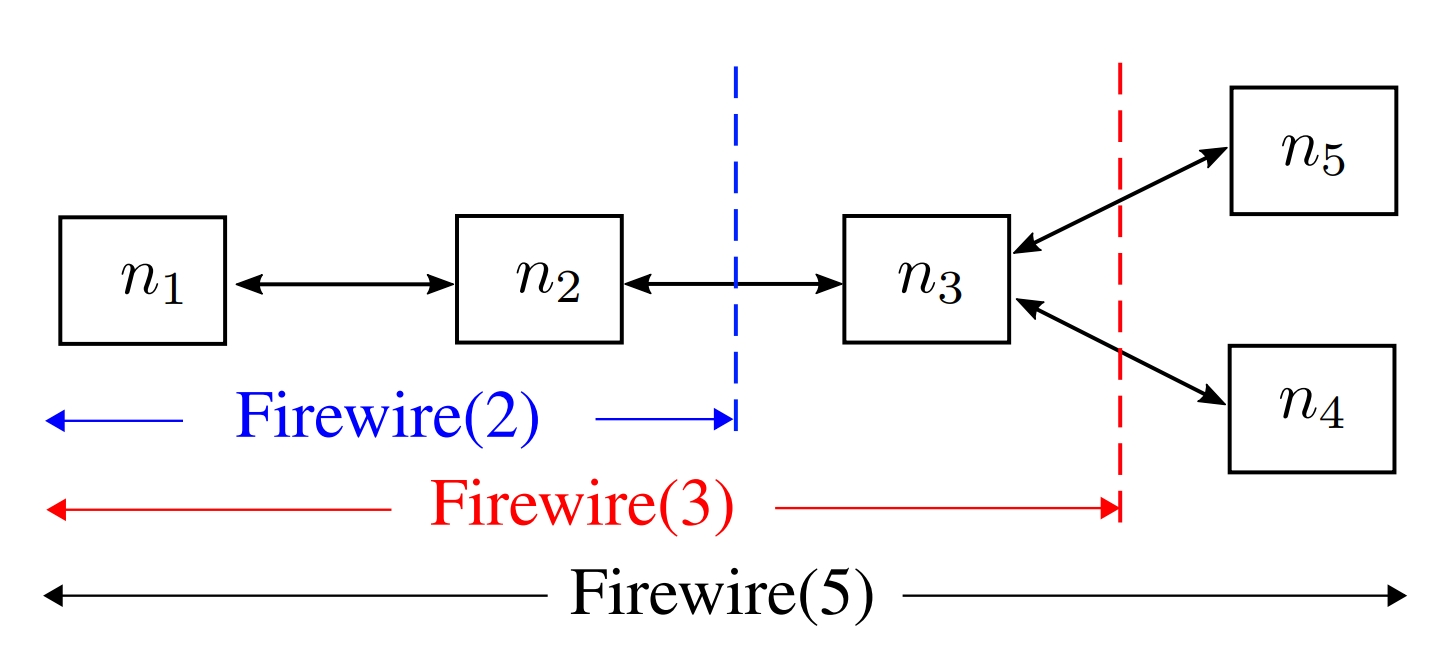
\includegraphics[scale=0.2]{Figures/firewireg}
\caption{FireWire Topologies with 2, 3 and 5 nodes}
\label{fig:fwg}
\end{figure}
The tree identification protocol is initiated by the leaf nodes of the topology. They send 
requests asking their neighbors to become their parents. A parent request sending mode is 
non deterministically chosen to be \emph{fast} or \emph{slow}. It determines the amount of time 
to wait before sending. Internal nodes of the topology keep on listening to parent requests 
until they receive exactly $n-1$ requests, $n$ being the number of neighbors. 
Then, they send a parent request
to their remaining neighbor. When receiving a parent request, a node either sends an 
acknowledgment, or detects a contention in the case it has also sent a parent request and it
is still waiting for an acknowledgment. Intuitively, a contention means that two neighbors are 
mutually asking to be leader. This situation is resolved by forcing both nodes to send new 
requests after a random waiting time.
We implemented a FireWire model inspired from the case-study in~\cite{firewire}, where the 
considered topology is made of two devices. 
Figure~\ref{fig:node} depicts the model for the node component.
\begin{figure}[!h]
 \centering
\begin{tikzpicture}[->,node distance=1.3cm,>=stealth',bend angle=20,auto,
  place/.style={circle,thick,draw=blue!75,fill=blue!20,minimum size=10mm},
  red place/.style={place,draw=red!75,fill=red!20}
  every label/.style={red},
  every node/.style={scale=.6},
  dots/.style={fill=black,circle,inner sep=2pt},
  initial text={}]

  \node [accepting, place,label=above:\textcolor{red}{$x\le 4$}] (l0)  {$\loc_0$};
  \node [place,below=1cm of l0,xshift=3cm,label=left:\textcolor{red}{$x\le 167$}] (l1) {$\loc_1$};
  \node [place,below=1cm of l0,xshift=-3cm,label=right:\textcolor{red}{$x\le 85$}] (l2) {$\loc_2$};
  \node [place,below=2.5cm of l0] (l3) {$\loc_3$};
  \node [place,below=1cm of l3, xshift=-3cm,label=below:\textcolor{red}{$x\le 4$}] (l4) {$\loc_4$};
  \node [place,below=1cm of l3,xshift=3cm] (l5) {$\loc_5$};
  \node [place,right=4cm of l3] (l6) {$\loc_6$};
  \node [place,left=4cm of l3] (l7) {$\loc_7$};
  
  
  \path (l0) edge node[sloped,midway,above]{$slow$} node[sloped,midway,below]{$x:=0$} (l1)
        (l0) edge node[sloped,midway,above]{$fast$}node[sloped,midway,below]{$x:=0$} (l2)
        (l1) edge node[sloped,midway,above]{$wait$}node[sloped,midway,below]{$159\le x\le167$} (l3)
        (l2) edge node[sloped,midway,above]{$wait$}node[sloped,midway,below]{$76\le x\le85$} (l3)
        (l2) edge [bend right] node[left,align=center]{$rcv\_req$\\$x:=0$} (l4)
        (l3) edge node[sloped,above, midway,align=center]{$rcv\_req$\\$x:=0$} (l4)
        (l3) edge node[sloped,above,midway,align=center]{$snd\_req$\\$x<=4$} (l5)
        (l5) edge[bend right=30] node[sloped,below,midway,align=center]{$rcv\_ack$} (l6)
        (l4) edge[bend left=30]node[sloped,below,midway]{$snd\_ack$} (l7);
        
        
  \draw[->] (l5) to[in=0,out=20,bend angle=30]node[sloped,above,midway]{$contention$} node[sloped,midway,below]{$x:=0$} (l0);
  \draw[->] (l6) to[in=10,out=90]node[sloped,above,midway]{$slave$}node[sloped,midway,below]{$x:=0$}  (l0);
  \draw[->] (l7) to[in=170,out=90]node[sloped,above,midway]{$leader$}node[sloped,midway,below]{$x:=0$}  (l0);
  \draw[->] (l1) to[bend left=25] node[sloped,above,midway,xshift=-1.2cm,yshift=2mm]{$rcv\_req$}node[sloped,midway,below,xshift=-1.2cm]{$x:=0$} (l4);
\end{tikzpicture}
  \caption{Timed Automaton for a Node}
 \label{fig:node}
\end{figure}  





\subsubsection{Gear Controller System}

The gear controller system (Figure~\ref{fig:gear}) describes the control system responsible 
for the gear change inside a
vehicle. The used model encompasses formal models of the gear controller and its environment.
The whole system includes five components: an interface, a controller, a clutch, an engine a
gear-box and two global variables. In order to change the gear, the interface sends a signal to 
the controller. Consequently, the controller interacts with the engine, the clutch and the 
gear-box to achieve the gear change. The engine is responsible of either regulating the torque 
or synchronizing the speed. On the other hand, the gear-box sets the gear between some fixed 
bounds, whereas, the clutch is used whenever the engine is not able to function properly 
(under difficult driving conditions, for instance). 
The case study was initially designed in UPPAAL~\cite{gear} and has been translated to BIP.
\begin{figure}[!h]
 \centering
\begin{tikzpicture}[
    dots/.style={fill=black,circle,inner sep=1pt},
  initial text={}]

\node (gc) [rectangle, draw=black, rounded corners, minimum width=30mm, minimum height=10mm] {Gear Controller};
\node (gb) [rectangle, draw=black, rounded corners, minimum width=30mm, minimum height=10mm,below=7.5mm of gc] {Gear Box};
\node (inf) [rectangle, draw=black, rounded corners, minimum width=30mm, minimum height=10mm,above=7.5mm of gc] {Interface};
\node (c) [rectangle, draw=black, rounded corners, minimum width=30mm, minimum height=10mm,below=7.5mm of gc, xshift=3.2cm] {Clutch};
\node (e) [rectangle, draw=black, rounded corners, minimum width=30mm, minimum height=10mm,below=7.5mm of gc, xshift=-3.2cm] {Engine};

  \node (i1) at ($(gc.north west)!0.7!(gc.north east)$) {};
  \node (i2) at ($(gc.north west)!0.3!(gc.north east)$) {};

  \node (i3) at ($(inf.south west)!0.7!(inf.south east)$) {};
  \node (i4) at ($(inf.south west)!0.3!(inf.south east)$) {};
  
  \draw[->] (i1.center) -- (i3.center);
  \draw[->] (i4.center) -- (i2.center);

  \node (i1) at ($(gb.north west)!0.7!(gb.north east)$) {};
  \node (i2) at ($(gb.north west)!0.3!(gb.north east)$) {};

  \node (i3) at ($(gc.south west)!0.7!(gc.south east)$) {};
  \node (i4) at ($(gc.south west)!0.3!(gc.south east)$) {};
  
  \draw[->] (i1.center) -- (i3.center);
  \draw[->] (i4.center) -- (i2.center);

  \node (i1) at ($(gc.north west)!0.7!(gc.south west)$) {};
  \node (i2) at ($(gc.north west)!0.3!(gc.south west)$) {};

  \node (i3) at ($(e.north west)!0.7!(e.north east)$) {};
  \node (i4) at ($(e.north west)!0.3!(e.north east)$) {};
  
  \draw[->] (i1.center) -| (i3.center);
  \draw[->] (i4.center) |- (i2.center);
  
  \node (i1) at ($(gc.north east)!0.7!(gc.south east)$) {};
  \node (i2) at ($(gc.north east)!0.3!(gc.south east)$) {};

  \node (i3) at ($(c.north west)!0.3!(c.north east)$) {};
  \node (i4) at ($(c.north west)!0.7!(c.north east)$) {};
  
  \draw[->] (i1.center) -| (i3.center);
  \draw[->] (i4.center) |- (i2.center);
\end{tikzpicture}
  \caption{Gear Controller System}
 \label{fig:gear}
\end{figure}  



The complete model (taken form~\cite{gear}) can be found in Appendix~\ref{ap1}.
\begin{remark}
Note that since the gear controller system contains to global variables, we had to tweak the 
generated invariants of the RTD-Finder tool as well as some of the predicates in order to 
restrict the set of reachable states of the system.
\end{remark}

\subsection{Results}
The experiments have been conducted on a HP machine with Ubuntu 16.04, an 
Intel\textsuperscript{\textregistered} Core\textsuperscript{\texttrademark}i5-4300U
processor of frequency 1.90GHz×4, and 7.7GiB memory.
\subsubsection{Conflict Detection Optimization}

\begin{table}[H]
  \caption{Experimental results}
    \label{tab:res}
  \begin{center}
\begin{tabular}{| l || c | c | c | c | c | c | c |}
    \hline
    Model                              & $n$                      & $i$                    & $c$          & $p$   & $f$   & $g$    & $t$   \\ \hline \hline                                  
    \multirow{14}{*}{Task Manager}     & 4                        & 8                      & 2            & 4     & 3     &  75\%  & 60.55ms \\ \cline{2-7}
                                       & \multirow{3}{*}{12}      & \multirow{3}{*}{40}    & 2            & 40    & 30    &  75\%  & 367.19ms \\ \cline{4-7}
                                       &                          &                        & 5            & 64    & 48    &  75\%  & 521.45ms \\ \cline{4-7}
                                       &                          &                        & 10           & 68    & 51    &  75\%  & 545.34ms \\ \cline{2-7}
                                       & \multirow{3}{*}{22}      & \multirow{3}{*}{80}    & 2            & 80    & 60    &  75\%  & 2.14s \\ \cline{4-7}
                                       &                          &                        & 10           & 144   & 108   &  75\%  & 3.41s \\ \cline{4-7}
                                       &                          &                        & 20           & 148   & 111   &  75\%  & 3.69s \\ \cline{2-7}
                                       & 32                       & 120                    & 30           & 228   & 171   &  75\%  & 8.41s \\ \cline{2-7}
                                       & 42                       & 160                    & 40           & 308   & 231   &  75\%  & 20.72s \\ \cline{2-7}
                                       & \multirow{6}{*}{52}      & \multirow{6}{*}{200}   & 2            & 200   & 150   &  75\%  & 22.56s \\ \cline{4-7}
                                       &                          &                        & 5            & 320   & 240   &  75\%  & 34.78s \\ \cline{4-7}
                                       &                          &                        & 10           & 360   & 270   &  75\%  & 37.72s \\ \cline{4-7}
                                       &                          &                        & 25           & 384   & 288   &  75\%  & 41.69s \\ \cline{4-7}
                                       &                          &                        & 50           & 388   & 291   &  75\%  & 45.35s \\ \cline{4-7}\hline
    \makecell{Train Gate\\Controller}  & 22                       & 45                     & 20           & 74    & 37    &  50\%  & 813,62ms \\ \hline
    \makecell{Gear \\Controller}       & 5                        & 32                     & 4            & 8     & 3     &  37.5\%  & 5,94s \\ \hline

  \end{tabular}
\end{center}
\end{table}
Table~\ref{tab:res} summarizes for each experiment the number of components ($n$), 
interactions ($i$),
partition classes ($c$), potential conflicts ($p$), false conflicts ($f$), the gain of the 
conflict detection 
and gives also the total verification time of our methods combined.
The above results give an indication on how much conflict resolution will be needed during 
execution. 

We first performed several experiments on different variants of the Task Manager example 
(with 2, 10, 20, 30, 40 and 50 Tasks). Each variant was tested with different partitioning of
interaction (different number of classes). Note that each time we chose the interaction
partition such that it yield the maximum number of potential conflicts. 
We can notice from the Task Manger experiments that increasing the number of interaction 
partition classes will increase the number of potential conflicts, that is,
the more distributed the system is the more conflicts it contains. 
Remark  that the percentage of gain remains the same meaning that our detection method
is not affected by the partitioning but rather bu the overall structure and dynamics of 
a given system.

We performed other experiments on real-life case studies such as the Train Gate Controller 
and the Gear Controller Systems which also yield interesting results in term of conflict 
detection ratio and execution time.

\subsubsection{Action-Time-Lock Detection for the \lpsabr}

Table~\ref{t:1} depicts the values $h_{\max}$ for each interaction of the Task Manager example, 
obtained while fixing $h_{\min}$.
Notice that the symmetry of the system implies the same $h_{\max}$ for interactions 
$\alpha_i,\alpha_{i+1},i\in\{1,3,5,7\}$. 
By remarking that location $\loc_3^2$ (resp. $\loc_3^3$) has a time progress condition 
$x\le4$ (resp. $y\le4$), and by observing that the clock $x$ is reset on the transition 
leading to this location, we can conclude that planning
the system with $h_{\min}>4$ will lead to an action-time-lock.
Particularly, in Example~\ref{exp:dl}, for $h_{\min}=2$ interaction $\alpha_6$ was planned 
with a horizon $\delta=8$, and consequently, leads to a action-time-lock state. Our method 
detects such cases and thus, finds that the maximum horizon for this interaction is 7. 
Likewise, the $h_{\max}$ for interactions $\alpha_2, \alpha_4\text{ and }\alpha_8$ 
(resp. $\alpha_1, \alpha_3\text{ and }\alpha_7$)
is found to be unbounded ($+\infty$).

\begin{table}[H]
  \caption{Detailed Results of the Task Manager Experiments}\label{t:1}
  \centering
  %  \vspace*{3mm}
  \begin{tabular}{| c || c | c | c | c |}
    \hline
    $h_{\min}$ & $\hmxb{\alpha_1}$, $\hmxb{\alpha_2}$ & $\hmxb{\alpha_3}$, $\hmxb{\alpha_4}$ & $\hmxb{\alpha_5}$, $\hmxb{\alpha_6}$  & $\hmxb{\alpha_7}$, $\hmxb{\alpha_8}$\\ \hline
        4      &                $+\infty$                    &                 $+\infty$                   &                9                     &               $+\infty$                 \\\hline
        3      &                $+\infty$                    &                 $+\infty$                   &                8                     &               $+\infty$                 \\\hline
        2      &                $+\infty$                    &                 $+\infty$                   &                7                     &               $+\infty$                 \\\hline
        1      &                $+\infty$                    &                 $+\infty$                   &                6                     &               $+\infty$                 \\\hline
  \end{tabular}
\end{table}

Table~\ref{t:2} summarizes the experiments obtained on the benchmarks stated above, where $n$ is
the number of components, $nb_{\I}$ the number of time progress conditions that will be 
verified
against action-time-lock freedom and
$\max h_{\min}$ the maximum value of $h_{\min}$ for which the system is action-time-lock-free in 
the planning semantics.
Additionally, the column $h_{\max}$ indicates whether a restriction on the upper horizons is 
required to avoid
deadlocks. Finally, $t_{exec}$ gives an overview of the execution time including both the 
invariants generation and the verification time.

\begin{table}[H]
  \caption{Experiments Results}\label{t:2}
 %   \vspace*{3mm}
  \centering
  \begin{tabular}{| c || c| c | c | c | c | c |}
  \hline
    Model                              & $n$ & $nb_{\I}$&  $\max h_{\min}$ &   $h_{\max}$ & $t_{exec}(s)$ \\\hline 
    Task Manager                       & 4  & 4  & 4            &  B         & 0.11 \\\hline 
    Train Gate Controller              & 3  & 6  & 4            &  $+\infty$        & 0.16   \\\hline 
    Firewire                           & 4  & 10 & 5            &  $+\infty$        & 3.03   \\\hline 
    Gear Controller                     & 5  & 19 & 130          &  $+\infty$        & 4.65    \\\hline 
  \end{tabular}
\end{table}

As shown in table~\ref{t:1}, the task manager model has a maximal $\hmin$ value of 4 TU 
and requires a restriction
on the upper horizons for interactions $\alpha_5$ and $\alpha_6$.
In the same way, we found that the train gate controller, the firewire and the train gate 
controller models have respectively maximal $\hmin$ value 
of 4 TU, 5 TU and 130 TU. However, they do not require any restriction on the upper 
horizons values of their interactions.




